\section{Data}
% are all the acronyms too much?
% TODO time and diurnal (?)
% TODO figure for regions
% TODO rainfall data
\begin{table}
  \centering
  \resizebox{0.85\linewidth}{!}{%
  \begin{tabular}{ l c c c }
    \toprule
    Channel & $\lambda_{\mathrm{cen}}$ ($\mu$m) & $\lambda_{\mathrm{min}}$ ($\mu$m) & $\lambda_{\mathrm{max}}$ ($\mu$m) \\
    \midrule
    VIS0.6  & 0.64                    & 0.56                    & 0.71                    \\
    VIS0.8  & 0.81                    & 0.74                    & 0.88                    \\
    NIR1.6  & 1.64                    & 1.50                    & 1.78                    \\
    \bottomrule
  \end{tabular}}
  \caption{Spectral characteristics of the three SEVIRI channels used
    in our work. Shown are the central, minimum and maximum
    wavelengths for the three spectral bands that we use.}
  \label{tab:seviri}
\end{table}

This work mainly comprises of analysing data products that we have
produced using raw data from the European Organisation for the
Exploitation of Meteorological Satellites
(EUMETSAT) \footnote{\url{https://www.eumetsat.int}}. In particular,
we have utilised the Meteosat Second Generation (MSG) series of
meterological satellites, which provide continous observations of the
full disk of the Earth via the Spinning Enhanced Visible and Infrared
Imager (SEVIRI) \citep{schmetz2002}. MSG is in an equatorial
geostationary orbit fixed at $0^{\circ}$ longitude and makes observations
every 15 minutes in 12 spectral bands, returning images $3712 \times 3712$
pixels in size. Not all of the 12 available bands are useful for our
investigation -- the spectral responses of the three bands that we use
are detailed in Table \ref{tab:seviri}. For consistency, we use data
collected at 12:00 each day, since this is the time when land is the
most illuminated.

\begin{table}
  \centering
  \resizebox{\linewidth}{!}{%
  \begin{tabular}{ l c c c c }
    \toprule
    \multirow{2}{*}{Region} &
    \multicolumn{2}{c}{Latitude (deg)} &
    \multicolumn{2}{c}{Longitude (deg)} \\
                 & {Top} & {Bottom} & {Left} & {Right}    \\
    \midrule
    South Africa & $-21.501$ & $-35.659$ & 14.728 & 33.193 \\
    East Africa  & 10.085    & 1.615     & 34.518 & 46.071 \\
    \bottomrule
  \end{tabular}}
  \caption{The coordinates that define our regions of interest. Top
    (Left) and Bottom (Right) correspond to the most northern
    (eastern) and southern (western) latitudes (longitudes) of the
    boxes defining the regions, respectively. All values in decimal
    degrees.}
  \label{tab:regions}
\end{table}

The full Earth image as collected by EUMETSAT is not terribly useful
in its original form for two reasons:
\begin{itemize}
  \item{it is quite a large
    image and so memory considerations alone make processing the whole
    image a difficult task;}
  \item{any effect that \elnino\ has on African climate is likely to be
    quite localised and, at the very least, we expect the trends to be
    reversed on either side of the equator.}
\end{itemize}
To address these challenges, we have defined two regions of interest
(selected after \cite{anyamba1996, anyamba2002}) in southern and
eastern Africa. The exact boundaries of these regions are listed in
Table \ref{tab:regions}. In addition, since we will be investigating
vegetation coverage, we restrict our study to continental areas using
the land mask provided by EUMETSAT.
\begin{figure}
  \centering
  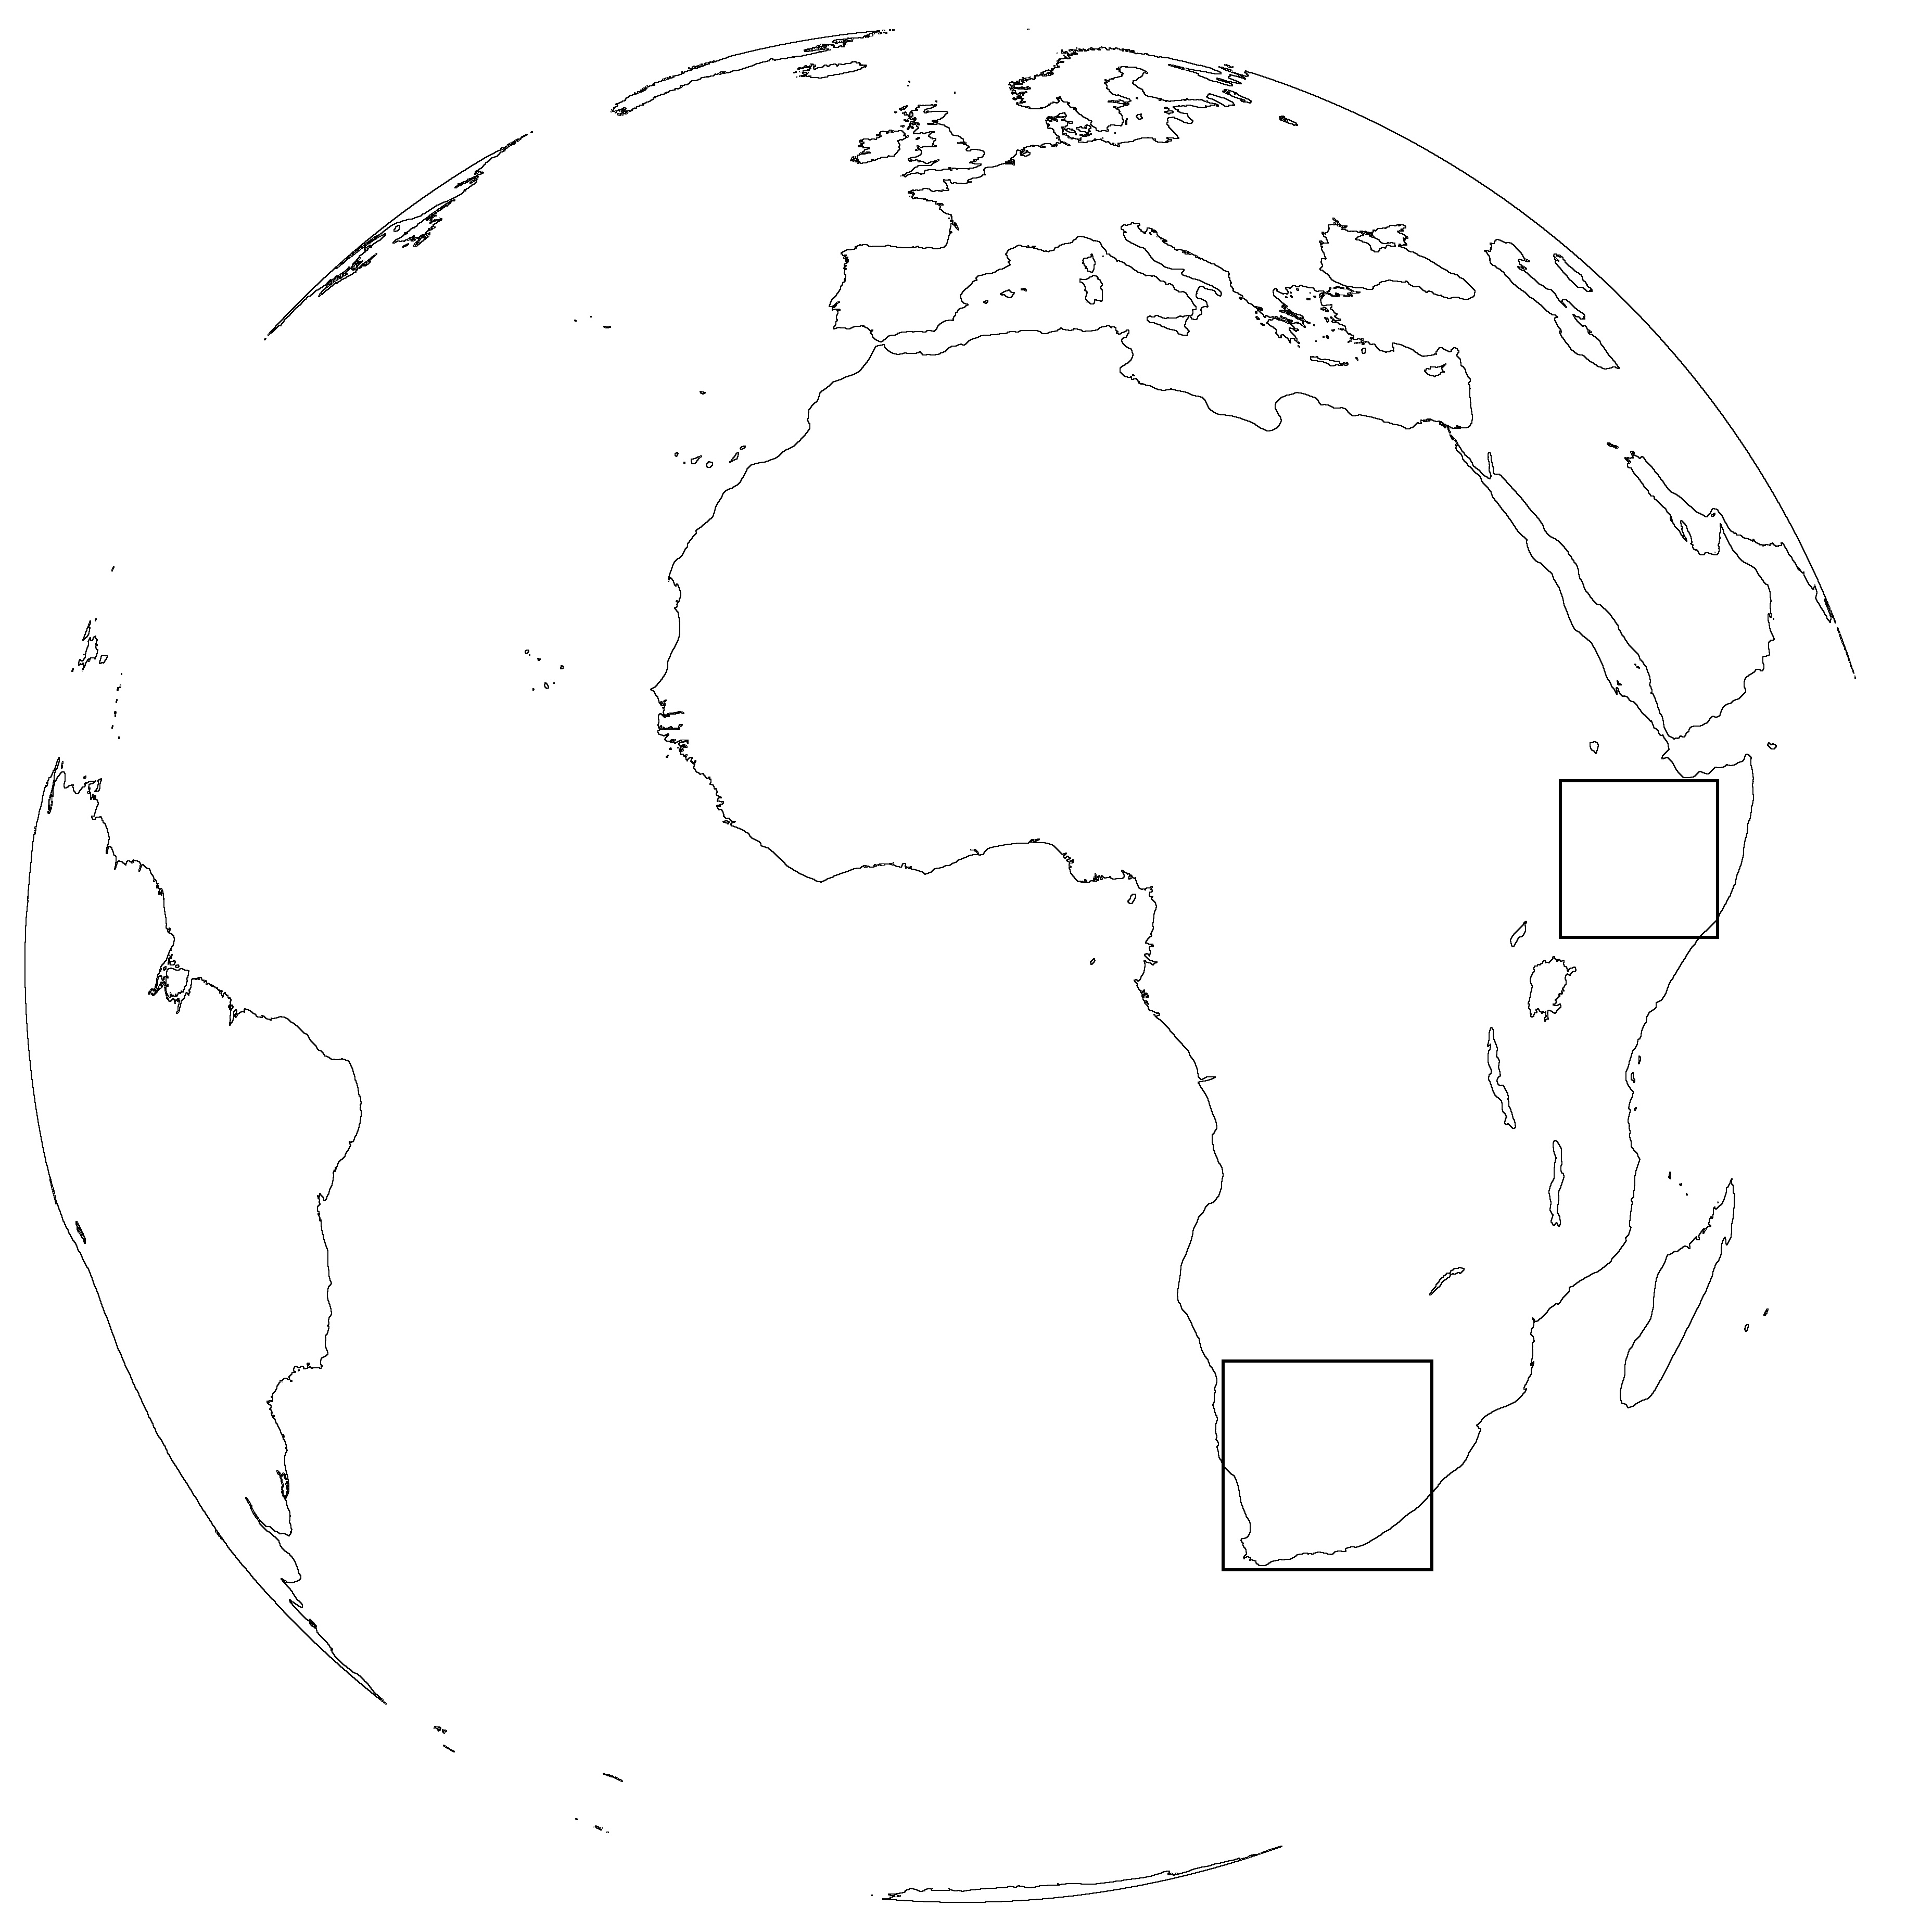
\includegraphics[width=0.9\linewidth]{figures/regions_figure}
  \caption{The EUMETSAT land mask image after using Sobel kernels to
    detect edges. The two black squares indicate the regions defined
    in Table \ref{tab:regions}.}
  \label{fig:regions}
\end{figure}
We also make use of data provided from other sources. For sea surface
temperature (SST) anomalies, we use the time series anomalies provided
by the National Oceanic and Atmospheric Administration
(NOAA) \footnote{\url{https://stateoftheocean.osmc.noaa.gov/}}. NOAA
provide SST anomalies for the Indian Ocean (IO) in the South Western
(SWIO) and Western Tropical (WTIO) regions, as well as Ni{\~n}o 3.4
SST anomalies. SWIO and WTIO anomalies are smoothed by taking three
month means, and the SWIO anomalies are compared to the data for South
Africa while the WTIO anomalies are compared to East Africa. We use
the anomalies in this way because each IO region is in close proximity
to its corresponding continental region, so it is reasonable to expect
that the anomalies may directly impact the continental climate. The
Ni{\~n}o 3.4 anomalies can be processed into the Oceanic Ni{\~n}o
Index (ONI) by smoothing with three monthly means, much in the same
way as the IO anomalies. \elnino\ events are then said to occur when
the ONI surpasses $0.5^{\circ}$C for at least five consecutive three
monthly periods. \nina\
conditions are present when the ONI falls
below $-0.5^{\circ}$C for the same time conditions.

The final tool in our complement of climate measures is rainfall
data. This is provided by the World
Bank \footnote{\url{http://www.worldbank.org/}} and we use it to
examine the extent to which cloud coverage is useful as a proxy
measure for rainfall.
